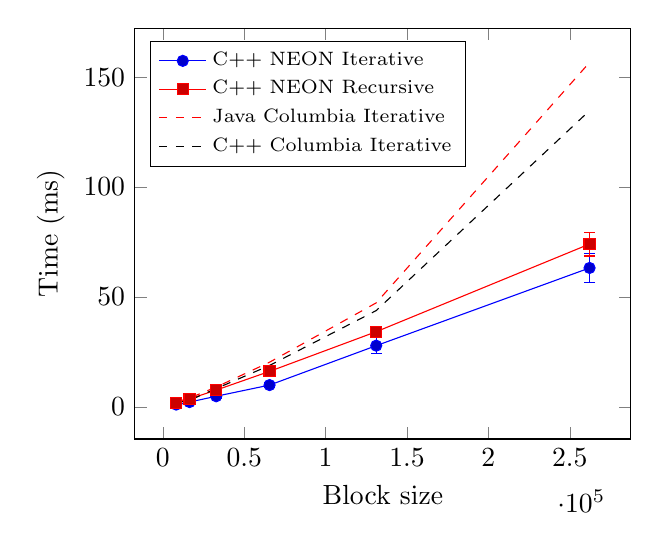
\begin{tikzpicture}
\begin{axis}[xlabel={Block size},ylabel={Time (ms)},width=0.65\linewidth,legend pos=north west,scaled y ticks = false,legend cell align=left,legend style={font=\scriptsize}]
\addplot+[error bars/.cd, y dir=both,y explicit] coordinates {
(8192, 1.0051) +- (0.0657, 0.0657)
(16384, 2.1559) +- (0.2562, 0.2562)
(32768, 4.7898) +- (0.7872, 0.7872)
(65536, 9.8807) +- (1.2509, 1.2509)
(131072, 27.8158) +- (3.6457, 3.6457)
(262144, 63.1858) +- (6.4595, 6.4595)
};
\addplot+[error bars/.cd, y dir=both,y explicit] coordinates {
(8192, 1.6133) +- (0.1416, 0.1416)
(16384, 3.5690) +- (0.4367, 0.4367)
(32768, 7.6009) +- (0.9583, 0.9583)
(65536, 16.1129) +- (1.8936, 1.8936)
(131072, 34.1650) +- (2.4085, 2.4085)
(262144, 74.0746) +- (5.4424, 5.4424)
};
\addplot+[style=dashed,color=red,mark=none] coordinates {
(8192, 2.1766) +- (0.3256, 0.3256)
(16384, 3.9995) +- (0.4596, 0.4596)
(32768, 8.9846) +- (1.3089, 1.3089)
(65536, 20.2833) +- (2.4423, 2.4423)
(131072, 47.2950) +- (6.6700, 6.6700)
(262144, 156.7135) +- (6.0892, 6.0892)
};
\addplot+[style=dashed,color=black,mark=none] coordinates {
(8192, 1.8030) +- (0.9841, 0.9841)
(16384, 2.9629) +- (0.6687, 0.6687)
(32768, 8.2847) +- (1.2061, 1.2061)
(65536, 18.8158) +- (2.8032, 2.8032)
(131072, 43.7807) +- (6.4454, 6.4454)
(262144, 134.8093) +- (10.2633, 10.2633)
};
\legend{C++ NEON Iterative , C++ NEON Recursive, Java Columbia Iterative, C++ Columbia Iterative}
\end{axis}
\end{tikzpicture}
